\subsection{Скорость звука в воздухе и воде. Особенности распространения звука в атмосфере и океане. Акустические методы исследования атмосферы.}
В линейном приближении без учёта вращения Земли уравнения движения (\ref{eq-2-2-2}) и неразрывности (\ref{eq-2-2-3}) имеют вид \cite{Носов-2019-14}:
\begin{equation}\label{eq-3-11-1}
\begin{cases}
\frac{\partial\vec{v}}{\partial t}=\vec{g}-\frac{\vec{\nabla}p}{\rho}
\\
\frac{\partial\rho}{\partial t}+\vec{\nabla}\cdot(\rho\vec{v})=0
\end{cases}
\end{equation}

Допустим следующие предположения \cite{Носов-2019-14}:
\begin{enumerate}
\item $\vec{v}=\vec{v}_0+\vec{v}_1$, где $\vec{v}_1$ -- малая величина. Для простоты будем считать $\vec{v}_0=0$.
\item $p=p_0+\widetilde{p}$, где $\widetilde{p}$ -- малая величина.
\item $\rho=\rho_0+\widetilde{\rho}$, где $\widetilde{\rho}$ -- малая величина.
\end{enumerate}

С учётом этих предположений и приближения гидростатики (\ref{eq-2-3-1}) система уравнений (\ref{eq-3-11-1}) преобразуется к:
\begin{equation}\label{eq-3-11-2}
\begin{cases}
\frac{\partial\vec{v}_1}{\partial t}=-\frac{\vec{\nabla}\widetilde{p}}{\rho_0}
\\
\vec{g}-\frac{\vec{\nabla}p_0}{\rho_0}=0
\\
\frac{\partial\widetilde{\rho}}{\partial t}+\rho_0\vec{\nabla}\vec{v}_1=0
\end{cases}
\end{equation}

Согласно Лапласу, вариации плотности $\widetilde{\rho}$ связаны с вариациями давления $\widetilde{p}$ соотношением:
\begin{equation}\label{eq-3-11-3}
\widetilde{\rho}=\left(\frac{\partial\rho}{\partial p}\right)_s\widetilde{p}=\left(\frac{1}{c_s^2}\right)\widetilde{p}
\end{equation}
где $c_s$ -- скорость звука\footnote{В воздухе зависимость $c_s=\sqrt{\frac{C_p}{C_V}R_{\mu}T}\approx340\,\text{м/c}$ аналитическая (определяется только температурой), а в воде зависимость $c_s=c_s(p, s, T)\approx1500\,\text{м/c}$ эмпирическая.}.

Подставляем (\ref{eq-3-11-3}) в (\ref{eq-3-11-2}) $\rightarrow$ дифференцируем первое уравнение по пространству ($\vec{\nabla}$), а третье по времени ($\frac{\partial}{\partial t}$) $\rightarrow$ вычитаем первое уравнение из третьего $\rightarrow$ получаем акустическое волновое уравнение относительно вариаций давления $\widetilde{p}$:
\begin{equation}
\frac{\partial^2\widetilde{p}}{\partial^2t}+c_s^2\Delta\widetilde{p}=0
\end{equation}

Наличие минимума в профиле скорости звука (см. рис. \ref{fig:c_s(h)}) обуславливает возможность захвата (образования \textit{подводного звукового канала}\footnote{Позволяет акустическим волнам распространяться минимальными потерями на большие расстояния.}) акустических волн подводными хребтами\footnote{Подводный хребет -- область под водой с пониженной глубиной $\Leftrightarrow$ область под водой с пониженной скоростью распространения длинных волн.} \cite{Носов-2019-14}.

\begin{figure}[!ht]
\centering
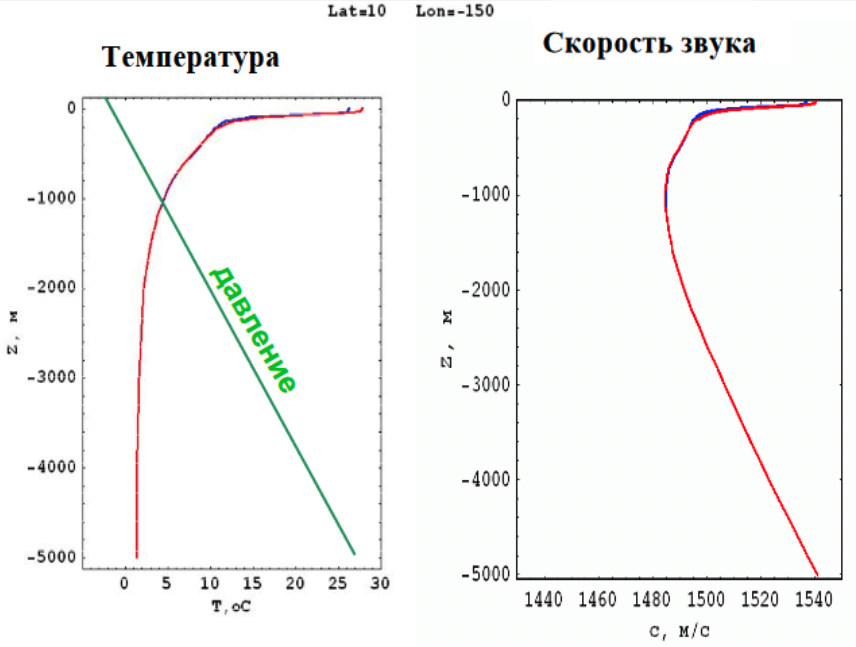
\includegraphics[width=0.4\textwidth]{images/c_s(h).png}
\caption{Профиль температуры (слева) и скорости звука (справа) в океане \cite{Носов-2019-14}.}\label{fig:c_s(h)}
\end{figure}

В приземном слое атмосферы при наличии температурной инверсии тоже может существовать своеобразный захват акустических волн (см. рис. \ref{fig:c_s(h)2}) \cite{Носов-2019-14}.
Так же в приземном слое атмосферы скорость ветра возрастает с высотой по логарифмическому закону (\ref{eq-4-4-1}).
Это обуславливает тот факт, что по направлению ветра звук распространяется дальше, чем против (см. рис. \ref{fig:c_s(h)2w}).

\begin{figure}[!ht]
\centering
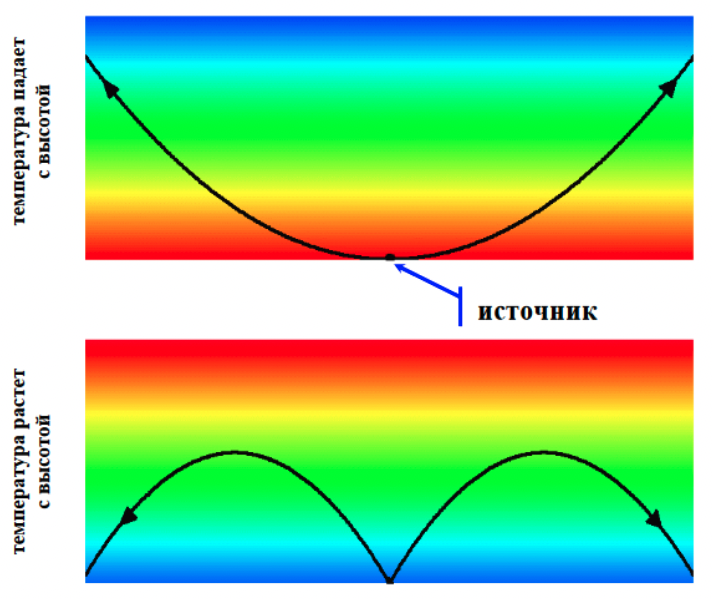
\includegraphics[width=0.4\textwidth]{images/c_s(h)2.png}
\caption{Профиль скорости звука в приземном слое атмосферы без (сверху) и при наличии (снизу) температурной инверсии \cite{Носов-2019-14}.}\label{fig:c_s(h)2}
\end{figure}

\begin{figure}[!ht]
\centering
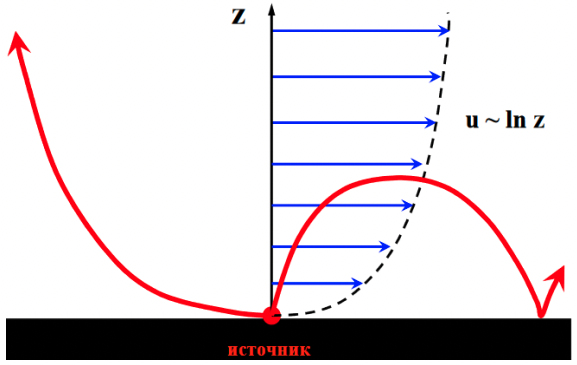
\includegraphics[width=0.4\textwidth]{images/c_s(h)2w.png}
\caption{Влияние скорости ветра на распространение звука в приземном слое атмосферы \cite{Носов-2019-14}.}\label{fig:c_s(h)2w}
\end{figure}
